%File: anonymous-submission-latex-2024.tex
\documentclass[letterpaper]{article} % DO NOT CHANGE THIS
\usepackage[submission]{aaai24}  % DO NOT CHANGE THIS
\usepackage{times}  % DO NOT CHANGE THIS
\usepackage{helvet}  % DO NOT CHANGE THIS
\usepackage{courier}  % DO NOT CHANGE THIS
\usepackage[hyphens]{url}  % DO NOT CHANGE THIS
\usepackage{graphicx} % DO NOT CHANGE THIS
\urlstyle{rm} % DO NOT CHANGE THIS
\def\UrlFont{\rm}  % DO NOT CHANGE THIS
\usepackage{natbib}  % DO NOT CHANGE THIS AND DO NOT ADD ANY OPTIONS TO IT
\usepackage{caption} % DO NOT CHANGE THIS AND DO NOT ADD ANY OPTIONS TO IT
\frenchspacing  % DO NOT CHANGE THIS
\setlength{\pdfpagewidth}{8.5in} % DO NOT CHANGE THIS
\setlength{\pdfpageheight}{11in} % DO NOT CHANGE THIS
%
% These are recommended to typeset algorithms but not required. See the subsubsection on algorithms. Remove them if you don't have algorithms in your paper.
\usepackage{algorithm}
\usepackage{algpseudocode}

%New Package
\usepackage{tablefootnote}
\usepackage{mathtools}
\usepackage{amsfonts}
\usepackage{multirow}
\usepackage{multicol}
\usepackage{booktabs}
\usepackage[dvipsnames]{xcolor}
\usepackage{adjustbox}
%
% These are are recommended to typeset listings but not required. See the subsubsection on listing. Remove this block if you don't have listings in your paper.
\usepackage{newfloat}
\usepackage{listings}
\DeclareCaptionStyle{ruled}{labelfont=normalfont,labelsep=colon,strut=off} % DO NOT CHANGE THIS
\lstset{%
	basicstyle={\footnotesize\ttfamily},% footnotesize acceptable for monospace
	numbers=left,numberstyle=\footnotesize,xleftmargin=2em,% show line numbers, remove this entire line if you don't want the numbers.
	aboveskip=0pt,belowskip=0pt,%
	showstringspaces=false,tabsize=2,breaklines=true}
\floatstyle{ruled}
\newfloat{listing}{tb}{lst}{}
\floatname{listing}{Listing}
%
% Keep the \pdfinfo as shown here. There's no need
% for you to add the /Title and /Author tags.
\pdfinfo{
/TemplateVersion (2024.1)
}

% DISALLOWED PACKAGES
% \usepackage{authblk} -- This package is specifically forbidden
% \usepackage{balance} -- This package is specifically forbidden
% \usepackage{color (if used in text)
% \usepackage{CJK} -- This package is specifically forbidden
% \usepackage{float} -- This package is specifically forbidden
% \usepackage{flushend} -- This package is specifically forbidden
% \usepackage{fontenc} -- This package is specifically forbidden
% \usepackage{fullpage} -- This package is specifically forbidden
% \usepackage{geometry} -- This package is specifically forbidden
% \usepackage{grffile} -- This package is specifically forbidden
% \usepackage{hyperref} -- This package is specifically forbidden
% \usepackage{navigator} -- This package is specifically forbidden
% (or any other package that embeds links such as navigator or hyperref)
% \indentfirst} -- This package is specifically forbidden
% \layout} -- This package is specifically forbidden
% \multicol} -- This package is specifically forbidden
% \nameref} -- This package is specifically forbidden
% \usepackage{savetrees} -- This package is specifically forbidden
% \usepackage{setspace} -- This package is specifically forbidden
% \usepackage{stfloats} -- This package is specifically forbidden
% \usepackage{tabu} -- This package is specifically forbidden
% \usepackage{titlesec} -- This package is specifically forbidden
% \usepackage{tocbibind} -- This package is specifically forbidden
% \usepackage{ulem} -- This package is specifically forbidden
% \usepackage{wrapfig} -- This package is specifically forbidden
% DISALLOWED COMMANDS
% \nocopyright -- Your paper will not be published if you use this command
% \addtolength -- This command may not be used
% \balance -- This command may not be used
% \baselinestretch -- Your paper will not be published if you use this command
% \clearpage -- No page breaks of any kind may be used for the final version of your paper
% \columnsep -- This command may not be used
% \newpage -- No page breaks of any kind may be used for the final version of your paper
% \pagebreak -- No page breaks of any kind may be used for the final version of your paperr
% \pagestyle -- This command may not be used
% \tiny -- This is not an acceptable font size.
% \vspace{- -- No negative value may be used in proximity of a caption, figure, table, section, subsection, subsubsection, or reference
% \vskip{- -- No negative value may be used to alter spacing above or below a caption, figure, table, section, subsection, subsubsection, or reference

\setcounter{secnumdepth}{0} %May be changed to 1 or 2 if section numbers are desired.

% The file aaai24.sty is the style file for AAAI Press
% proceedings, working notes, and technical reports.
%

% Title

% Your title must be in mixed case, not sentence case.
% That means all verbs (including short verbs like be, is, using,and go),
% nouns, adverbs, adjectives should be capitalized, including both words in hyphenated terms, while
% articles, conjunctions, and prepositions are lower case unless they
% directly follow a colon or long dash
\title{AAAI Press Anonymous Submission\\Instructions for Authors Using \LaTeX{}}
\author{
    %Authors
    % All authors must be in the same font size and format.
    Written by AAAI Press Staff\textsuperscript{\rm 1}\thanks{With help from the AAAI Publications Committee.}\\
    AAAI Style Contributions by Pater Patel Schneider,
    Sunil Issar,\\
    J. Scott Penberthy,
    George Ferguson,
    Hans Guesgen,
    Francisco Cruz\equalcontrib,
    Marc Pujol-Gonzalez\equalcontrib
}
\affiliations{
    %Afiliations
    \textsuperscript{\rm 1}Association for the Advancement of Artificial Intelligence\\
    % If you have multiple authors and multiple affiliations
    % use superscripts in text and roman font to identify them.
    % For example,

    % Sunil Issar\textsuperscript{\rm 2},
    % J. Scott Penberthy\textsuperscript{\rm 3},
    % George Ferguson\textsuperscript{\rm 4},
    % Hans Guesgen\textsuperscript{\rm 5}
    % Note that the comma should be placed after the superscript

    1900 Embarcadero Road, Suite 101\\
    Palo Alto, California 94303-3310 USA\\
    % email address must be in roman text type, not monospace or sans serif
    proceedings-questions@aaai.org
%
% See more examples next
}

%Example, Single Author, ->> remove \iffalse,\fi and place them surrounding AAAI title to use it
\iffalse
\title{My Publication Title --- Single Author}
\author {
    Author Name
}
\affiliations{
    Affiliation\\
    Affiliation Line 2\\
    name@example.com
}
\fi

\iffalse
%Example, Multiple Authors, ->> remove \iffalse,\fi and place them surrounding AAAI title to use it
\title{My Publication Title --- Multiple Authors}
\author {
    % Authors
    First Author Name\textsuperscript{\rm 1},
    Second Author Name\textsuperscript{\rm 2},
    Third Author Name\textsuperscript{\rm 1}
}
\affiliations {
    % Affiliations
    \textsuperscript{\rm 1}Affiliation 1\\
    \textsuperscript{\rm 2}Affiliation 2\\
    firstAuthor@affiliation1.com, secondAuthor@affilation2.com, thirdAuthor@affiliation1.com
}
\fi


% REMOVE THIS: bibentry
% This is only needed to show inline citations in the guidelines document. You should not need it and can safely delete it.
\usepackage{bibentry}
% END REMOVE bibentry

\begin{document}

\section{Technical Appendix}
For a better understanding, we provide auxiliary resources regarding our proposed EIISRS model in the appendix, including algorithm, complexity analysis, and additional case studies.
\section{A{\quad}Algorithm}
\begin{algorithm}[h]
    \caption{The first training epoch of EIISRS}
    \label{alg:algorithm}
    \textbf{Input}: user-item interaction matrix $\textbf{\textit{R}}$, social networks $\textbf{\textit{S}}$, and Gaussian random initialize user embeddings $\textbf{\textit{P}}^{(0)}$ and item embeddings $\textbf{\textit{Q}}^{(0)}$\\
    \textbf{Output}: user embeddings $\textbf{\textit{P}}_{final}$ and item embeddings $\textbf{\textit{Q}}$, augmented social networks $\widetilde{\textbf{\textit{S}}}$
    \begin{algorithmic}[1]
        \For{each iteration}
            \For{each batch}
                \State $\textbf{\textit{P}}^{(0)}_s, \textbf{\textit{P}}^{(0)}_r \gets$ Eq.(1); \textcolor{RoyalBlue}{\Comment{Self-gating Unit}}
                \For{$l=1:L$}
                    \State $\textbf{\textit{P}}^{(l)}_s$, $\textbf{\textit{P}}^{(l)}_r$, $\textbf{\textit{Q}}^{(l)}$ $\gets$ Eq.(2)-(4);\textcolor{RoyalBlue}{\Comment{Graph Conv.}}
                    \State $\boldsymbol{\mu}^{(l)}$, $\boldsymbol{\sigma}^{(1)} \gets$ Eq.(8);
                    \State $\textbf{\textit{z}}^{(l)} \gets$ Eq.(9); \textcolor{RoyalBlue}{\Comment{Social Diversity Simulation}}
                    \State $\boldsymbol{\alpha}_i \gets$ Eq.(5);
                    \State Calculate the $\mathcal{L}_{reconstruct}$ and $KLD$;
                \EndFor
                \State $\textbf{\textit{P}}_s = \sum_{i=0}^{L}\textbf{\textit{P}}_s^{(l)}$; \textcolor{RoyalBlue}{\Comment{Social Influence Propagation}}
                \State $\textbf{\textit{P}}_{final} \gets$ Eq.(14);
                \State Calculate the pairwise BPR loss $\mathcal{L}_{rec}$;
            \EndFor
            \State $\widetilde{\textbf{\textit{S}}} \gets$ Eq.(10)-(13); \textcolor{RoyalBlue}{\Comment{Social Influence Exploration}}
        \EndFor
        \State return $\textbf{\textit{P}}_{final}, \textbf{\textit{Q}}, \widetilde{\textbf{\textit{S}}}$
    \end{algorithmic}
\end{algorithm}
For the rest training epochs, we replace the social networks \textbf{\textit{S}} with augmented social networks $\widetilde{\textbf{\textit{S}}}$ as input.

\section{B{\quad}Complexity Analysis}
This section is going to talk about the model size and time complexity of our model.
\subsection{Model Size}
For model size, there are six parts that introduce trainable parameters: user/item embeddings, self-gating units, layerwise attention unit, selectors, encoder/decoder in LGE-VAE, and aggregation matrix. The size of user and item embeddings in total is $(m+n)\times d$. Each self-gating unit and layerwise attention unit occupied $(d+1)\times d$, altogether $3\times (d+1)$. $K$ selectors take up $k\times m$ in total. Encoder occupies $2\times d\times d$ while decoder is $d\times d$, same as the aggregation matrix. To sum up, the total size of our model is approximately equal to $(m+n+7d+3)\times d+ k\times m$. Owing to $d\ll min(m,n)$ and $k\ll m$, our model is fairly portable.
\subsection{Time Complexity}
For time complexity, analogously, there are also the six parts that cost our computational power. Regarding graph convolution, the time complexity is $\mathcal{O}(|\textbf{\textit{R}}^+|dL)$ for the user-item bipartite graph, and $\mathcal{O}(|\textbf{\textit{S}}^+|dL)$ for the social graph, where $|\textbf{\textit{R}}^+|$ and $|\textbf{\textit{S}}^+|$ denote the non-zero values of original graph respectively. Compared with previous graph-based recommendation systems, we drop out the feature transformation matrix and activation function, so the time complexity of graph convolution is relatively slower. For the self-gating units, layerwise attention unit, encoder/decoder of LGE-VAE, and aggregation matrix, the time complexity is as low as $\mathcal{O}(md^2)$. The most intractable time consumption is the selectors. Since we need to calculate the cosine similarity among all users, the time complexity used to be $\mathcal{O}(m^2d)$, where it would be exponentially increased along with the linear increment of our input data. To tackle this problem, for each epoch, we only choose a tiny subset of users $\mathcal{U}^+$ to do the processing, in which $|\mathcal{U}^+| \ll m$. After the two most time-consuming components, namely graph convolution and selectors, have been tailored without spoiling the effectiveness, our model is fairly efficient, too.

\section{C{\quad}Case Study}
This section exhibits some case studies of our model as supplements, in order to illustrate the validity of our hypothesis. For simplification, we take LastFM as an example. 
\subsection{Analysis of Implicit Social Graph}
\begin{figure}[ht!]
  \centering
  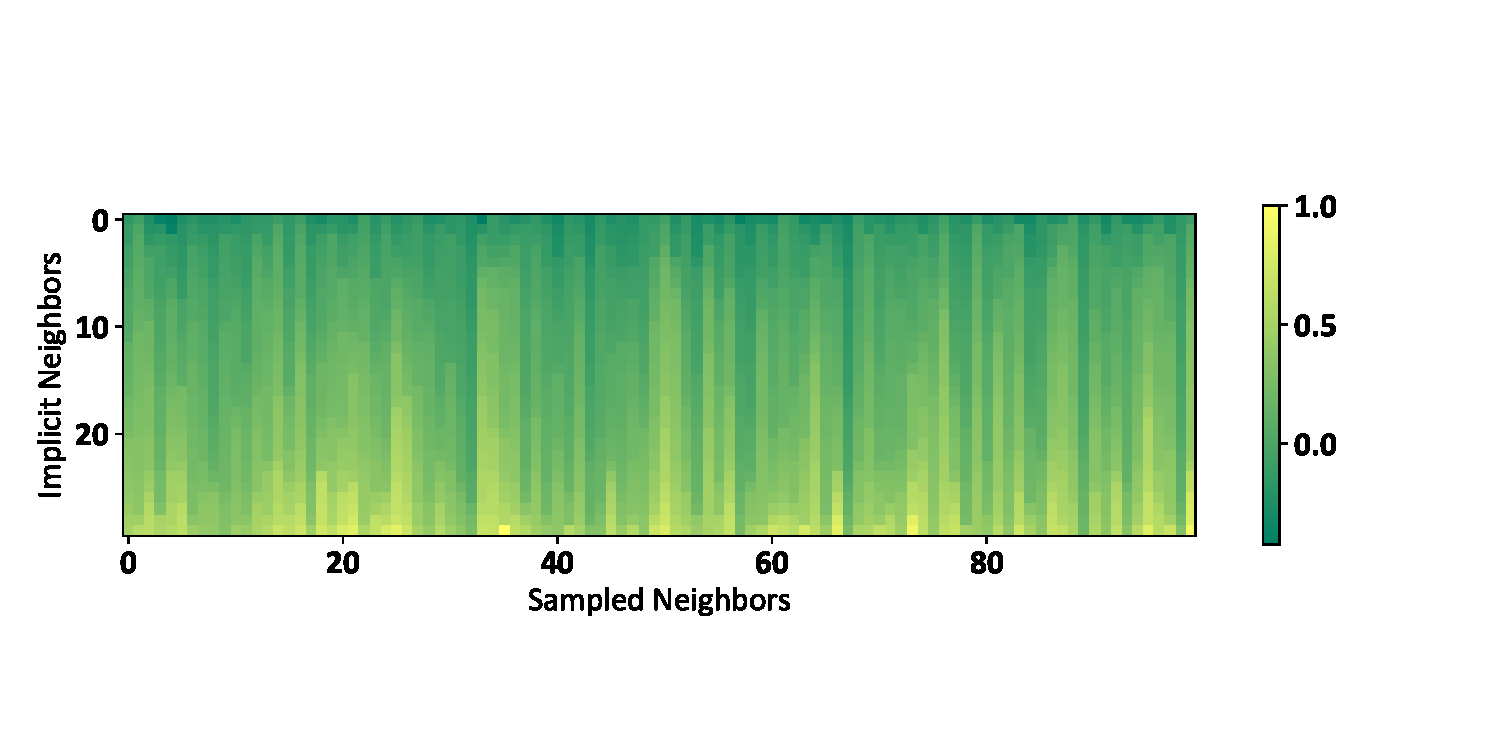
\includegraphics[width=0.5\textwidth]{implicit.pdf} %1.png是图片文件的相对路径
  \caption{Illustration of the similarity with implicit social neighbors.}
  \label{fig_implicit}
\end{figure}
\noindent As shown in Figure \ref{fig_implicit}, the color shows the similarity between sampled neighbors and generated implicit neighbors. The closer the score to 1, the more similar the two users are, and the lighter the color is. Vice versa. We can observe from the graph that different candidate neighbors have different similarities. We can make an inference that the implicit neighbors are not always highly similar to the sampled user since the anchor user probably has diverse interests and cannot be exactly assigned to an agminated neighborhood. It is also evidence of why we apply social diversity simulation in our model.

\subsection{Anlaysis of User Representation Collapse}
\subsection{Additional Comparison}

\end{document}
